\section{Ontology}
\label{sec:ontology}

Pada tahun 1993, \cite{gruber1993translation} pertama mendefinisikan sebuah ontology sebagai "\textit{explicit specification of a conceptualization}". Pada tahun 1997, \cite{borst1997construction} mendefinisikan ontology sebagai "\textit{formal specification of a shared conceptualization}". Definisi ini menambahkan kebutuhan sebuah ontology sebagai sebuah representasi konseptual yang \textit{shared} diantara beberapa pihak. Sehingga, konseptualisasi tersebut harus diekspresikan dengan sebuah format yang \textit{machine readable}. Sehingga pada tahun 1998, \cite{studer1998knowledge} menggabungkan kedua definisi tersebut sebagai "\textit{an ontology is a formal, explicit specification of a shared conceptualization}."

Dalam tulisannya, \cite{Guarino2009} merangkum ketiga definisi tersebut menjadi: Ontology adalah sebuah \textit{framework} terstruktur untuk merepresentasikan pengetahuan di sebuah \textit{domain} tertentu, seperti mendefinisikan entitas, konsep, dan relasi di dalam \textit{domain} tersebut. Ontology dapat membantu membuat sebuah model yang dapat dimengerti dan dapat dibagikan untuk digunakan dalam berbagai sistem dan aplikasi. Di dalam \textit{domain} sistem informasi, ontology digunakan sebagai sebuah cara formal untuk mengorganisasikan dan merepresentasikan data untuk dibagikan, dilakukan pencarian, dan dilakukan penalaran \parencite{Guarino2009}. 

Beberapa komponen kunci dari sebuah ontology adalah:

\begin{enumerate}
  \item \textit{Classes (Concepts)}: Tipe atau kategori fundamental di dalam sebuah \textit{domain} yang merepresentasikan konsep umum.
  \item \textit{Instances (Individuals)}: Contoh spesifik dari sebuah \textit{class}.
  \item \textit{Properties (Attributes)}: Mendeskripsikan karakteristik dari \textit{classes} atau \textit{instances}.
  \item \textit{Relationships}: Hubungan antar entitas, bisa \textit{hierarchical} atau \textit{associative}.
  \item \textit{Axioms}: Aturan atau \textit{constraint} yang mendefinisikan \textit{valid relationships} dan \textit{properties} di dalam ontology, sehingga dapat dilakukan inferensi logis.
\end{enumerate}

\subsection{The Semantic Web}
\label{subsec:the-semantic-web}

\textit{The Semantic Web} adalah sebuah ekstensi dari \textit{web} dengan tambahan data dengan arti yang terdefinisi dengan baik, yang diturunkan menggunakan \textit{semantic theory} untuk menginterpretasikan simbol-simbol. \textit{Semantic theory} menyediakan catatan dari arti untuk sebuah istilah atau informasi, sehingga dapat membuat sebuah hubungan logis antar istilah \parencite{shadbolt2006semantic}.

\subsubsection{Universal Resource Identifiers}
\label{subsubsec:universal-resource-identifiers}

\textit{Universal Resource Identifiers (URIs)} adalah sebuah cara untuk mengidentifikasi sebuah \textit{resource} menggunakan sebuah konvensi penamaan global yang disepakati, sehingga dapat diinterpretasikan secara standar oleh seluruh mesin yang berada di \textit{web}. Saat sebuah \textit{resource} diasosiasikan dengan sebuah URI, maka itu berarti semua orang dapat melakukan \textit{link}, \textit{refer}, dan mengambil \textit{representasi} dari \textit{resource} tersebut menggunakan URI. Skema yang direkomendasikan pada tahun 2004 adalah \textit{Resource Definition Framework Schema} yang menggunakan spesifikasi dasar dari RDF dengan ekstensi untuk mendukung ekspresi dari \textit{structured vocabularies} \parencite{shadbolt2006semantic}.

\subsubsection{Web Ontology Langugage}
\label{subsubsec:web-ontology-language}

\textit{Web Ontology Language (OWL)} adalah keluarga bahasa yang dikembangkan oleh \textit{World Wide Web Consortium (W3C)}, digunakan untuk mengembangkan dan berbagi ontology di dalam \textit{web}. OWL bertujuan untuk memberikan representasi yang efisien untuk ontology, pengecekan \textit{logical consistency} dan klasifikasi \textit{concept}, menggunakan RDF untuk \textit{linking} sehingga ontology dapat didistribusikan antar sistem \parencite{shadbolt2006semantic}.

\subsection{Ontology in Blockchain}
\label{subsec:ontology-in-blockchain}

Konsep ontology di dalam Blockchain adalah sebuah pendekatan yang berupaya untuk memetakan fitur dan konsep dari Blockchain secara formal dan \textit{shared} untuk mendukung \textit{interoperability} \parencite{9770809} dan mewujudkan visi \textit{semantic} Blockchain \parencite{hector2020blondie}. 

\subsubsection{EthOn}
\label{subsubsec:ethon}

\begin{figure}[ht]
  \centering
  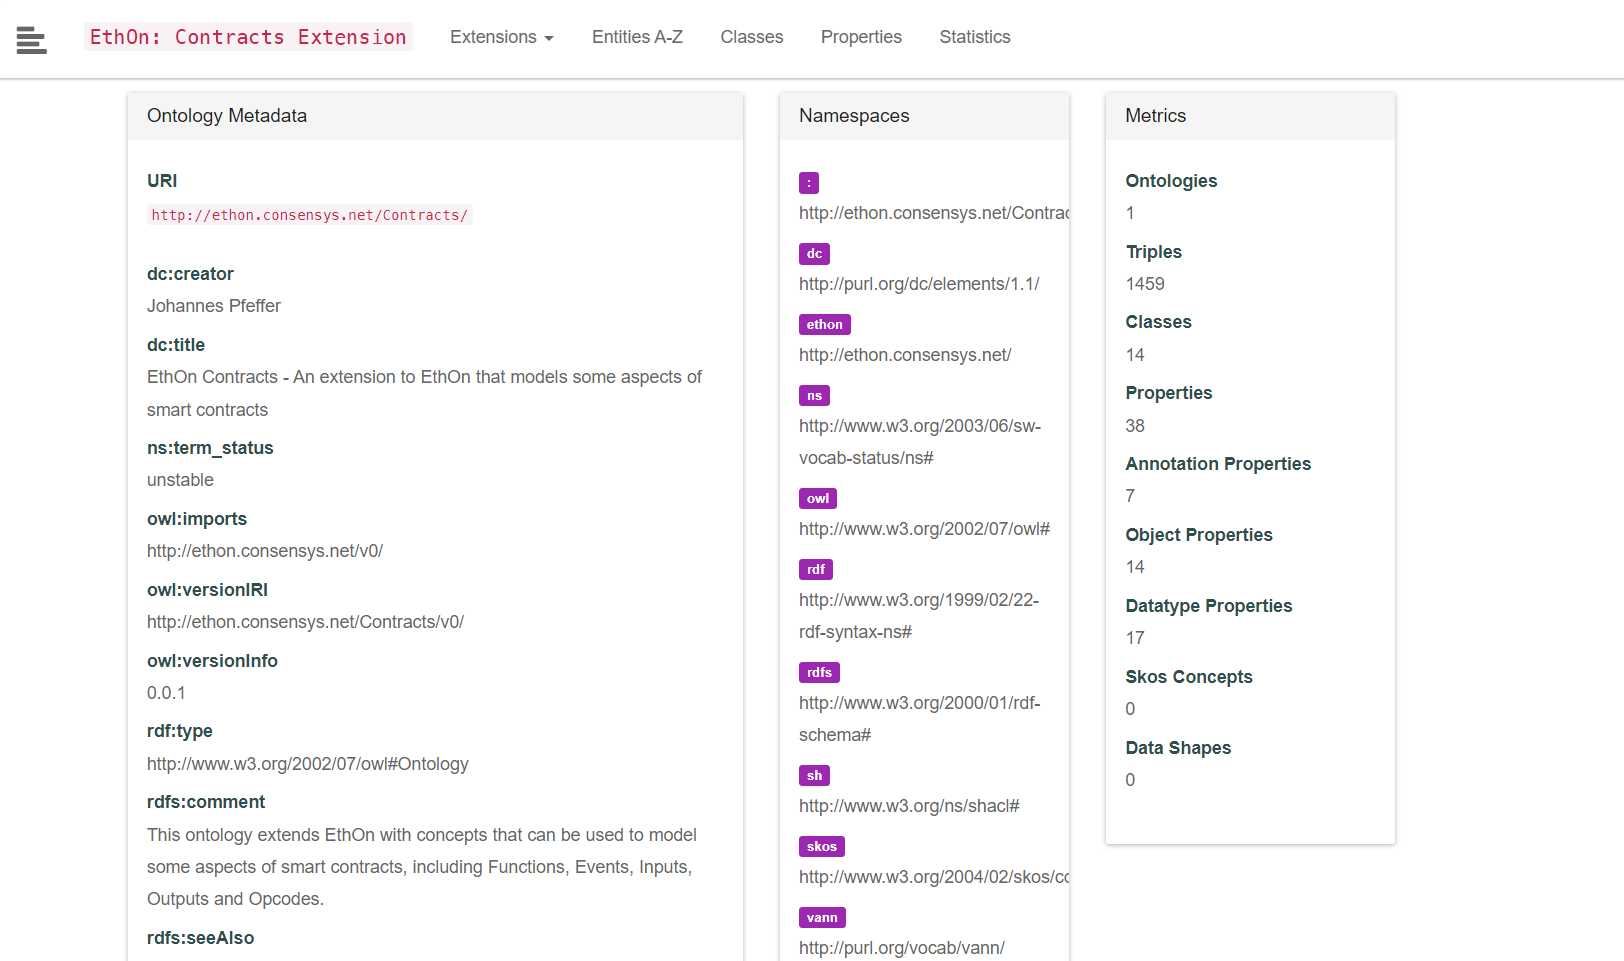
\includegraphics[width=0.7\textwidth]{resources/chapter-2/ethon.png}
  \caption{Visualisasi EthOn \parencite{ethon2024}}
  \label{image:ethon}
\end{figure}

EthOn adalah sebuah ontology yang dirancang secara spesifik untuk ekosistem Ethereum untuk merepresentasikan struktur, komponen, dan relasi di dalam Blockchain Ethereum. EthOn menyediakan \textit{semantic framework} untuk standarisasi dan interpretasi data kompleks yang terasosiasi dengan transaksi, Smart Contracts, blok, akun, dan entitas lainnya. Ontology ini memberikan cara untuk menginterpretasikan data dengan cara yang lebih terstruktur dan berarti, mendukung \textit{interoperability}, dan integrasi data \parencite{pfeffer2016ethon}.

\subsubsection{BLONDiE}
\label{subsubsec:blondie}

\begin{figure}[ht]
  \centering
  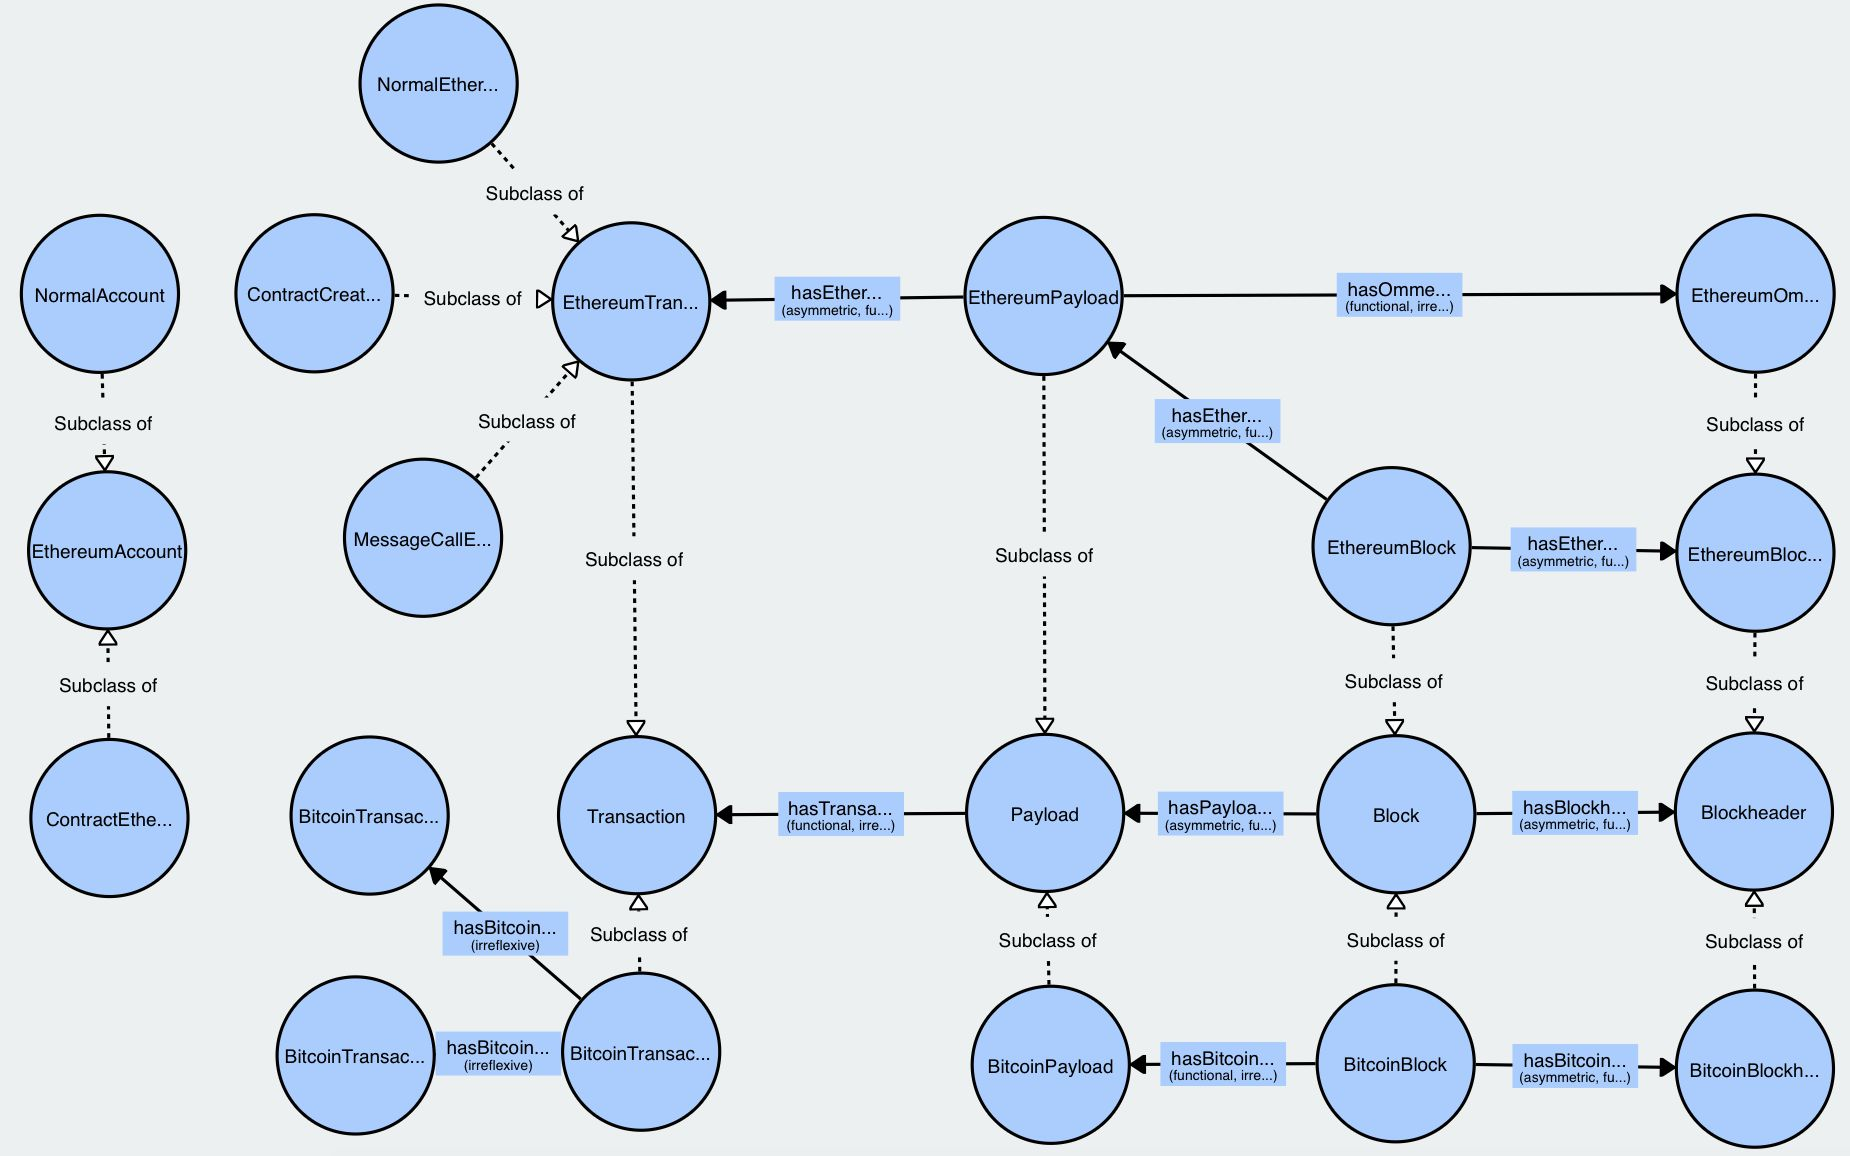
\includegraphics[width=1\textwidth]{resources/chapter-2/blondie-visualization.jpg}
  \caption{Visualisasi Ontologi BLONDiE \parencite{third2017linked}}
  \label{image:blondie-visualization}
\end{figure}

BLONDiE adalah singkatan dari Blockchain Ontology with Dynamic Extensibility, yang merupakan sebuah \textit{vocabulary} untuk merepresentasikan konsep di dalam Blockchain dengan potensi untuk ekstensi. Ontology ini terdiri atas 23 \textit{class}, 11 \textit{object properties}, dan 64 \textit{data properties} \parencite{hector2020blondie}. Gambar \ref{image:blondie-visualization} memvisualisasikan ontologi BLONDiE.

\subsection{Minimal Service Model}
\label{subsec:minimal-service-model}

Minimal Service Model adalah sebuah RDF(S) integration ontology sederhana berdasarkan prinsip \textit{minimal ontological commitment}, yaitu prinsip dalam perancangan ontology yang berarti membuat klaim atau asumsi sesedikit mungkin tentang domain yang dimodelkan. MSM hanya mendefinisikan struktur dasar seperti Services, Operations, dan Message Content. MSM dikembangkan bukan untuk menambah keragaman model \textit{service} yang sudah ada, melainkan berfungsi sebagai model untuk integrasi yang menjembatani berbagai formalisme yang telah ada. Model ini mampu menangkap semantik inti dari Web Service dan Web API dalam satu model yang sama, sehingga mendukung proses publikasi dan penemuan \textit{service} secara homogen. Salah satu fitur kunci dari MSM adalah kemampuan integrasinya, yang menggunakan properti msm untuk memungkinkan \textit{binding} ke berbagai format deskripsi untuk sebuah \textit{service} seperti WSDL, SWAGGER, WSMO, dan OWL-S, dan juga integrasi \textit{vocabulary} dari ontology lainnya \parencite{iserve2015datamodel}.

Ekstensi Minimal Service Model antara lain:
\begin{enumerate}
  \item MSM-WSDL \break Memberikan kemampuan \textit{grounding} ke elemen-elemen WSDL.
  \item MSM-SWAGGER \break Memberikan kemampuan \textit{grounding} untuk deskripsi SWAGGER.
  \item MSM-NFP \break Melacak metrik penggunaan \textit{service} yang mencakup informasi terkait properti non-fungsional.
\end{enumerate}

\begin{figure}[ht]
  \centering
  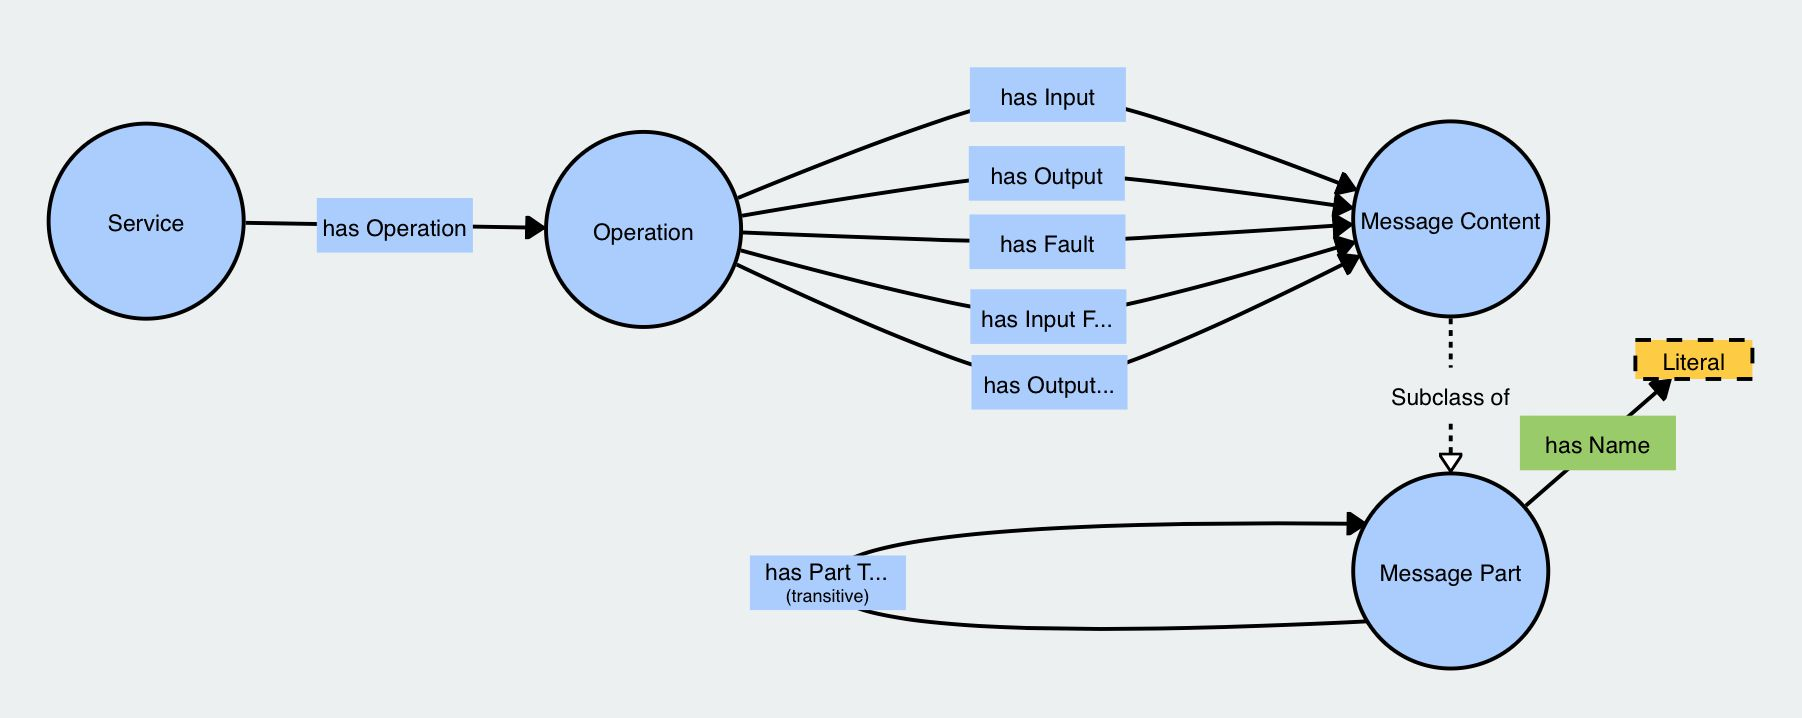
\includegraphics[width=1\textwidth]{resources/chapter-2/msm-visualization.jpg}
  \caption{Visualisasi Ontologi Minimal Service Model \parencite{third2017linked}}
  \label{image:msm-visualization}
\end{figure}